\documentclass{article}

% content/resources/templates/preamble.tex
\usepackage[margin=0.6in]{geometry}
\author{Milav Dabgar}
\usepackage{amsmath,amssymb,amsthm}
\usepackage{booktabs}
\usepackage{multirow}
\usepackage{xcolor}
\usepackage{tcolorbox}
\tcbuselibrary{breakable,skins}
\usepackage[colorlinks=true,linkcolor=blue]{hyperref}
\usepackage{titlesec}
\usepackage{enumitem}
\usepackage{tikz}
\usepackage{pgfplots}
\usepackage{circuitikz}
\usepackage[version=4]{mhchem}
\usepackage{longtable}
\usepackage{array}
\usepackage{float}
\usepackage{caption}
\usepackage{listings}

\lstset{
  basicstyle=\small\ttfamily,
  breaklines=true,
  breakatwhitespace=false,
  postbreak=\mbox{\textcolor{red}{$\hookrightarrow$}\space},
  float=false,
  numbers=left,
  numberstyle=\tiny\color{gray},
  numbersep=10pt,
  xleftmargin=2em,
  keywordstyle=\color{blue},
  commentstyle=\color{green!60!black},
  stringstyle=\color{purple},
  backgroundcolor=\color{gray!5},
  showstringspaces=false,
  tabsize=2,
  captionpos=b,
  keepspaces=true,
  columns=flexible
}

\pgfplotsset{compat=1.18}
\usetikzlibrary{shapes,arrows,positioning,calc,patterns,decorations.pathmorphing,decorations.markings,arrows.meta}

% Color scheme
\definecolor{headcolor}{RGB}{0,102,204}
\definecolor{keycolor}{RGB}{220,20,60}
\definecolor{solutioncolor}{RGB}{34,139,34}
\definecolor{mnemoniccolor}{RGB}{148,0,211}
\definecolor{codecolor}{RGB}{0,0,100}

% Spacing
\setlength{\parskip}{3pt}
\setlist[itemize]{nosep}
\setlist[enumerate]{nosep}

% Title formatting
\titleformat{\section}{\Large\bfseries\color{headcolor}}{\thesection}{1em}{}
\titleformat{\subsection}{\large\bfseries\color{headcolor}}{\thesubsection}{1em}{}

% Pandoc tightlist compatibility
\providecommand{\tightlist}{%
  \setlength{\itemsep}{0pt}\setlength{\parskip}{0pt}}

% Pandoc longtable compatibility
\newcounter{none}
\def\thenone{}


% content/resources/templates/english-boxes.tex

% Custom environments
\newtcolorbox{solutionbox}{
 breakable,
 enhanced,
 colback=solutioncolor!5!white,
 colframe=solutioncolor!75!black,
 fonttitle=\bfseries,
 title=Solution
}

\newtcolorbox{solutionboxnobreak}{
 colback=solutioncolor!5!white,
 colframe=solutioncolor!75!black,
 fonttitle=\bfseries,
 title=Solution
}

\newtcolorbox{keyformula}{
 breakable,
 enhanced,
 colback=keycolor!5!white,
 colframe=keycolor!75!black,
 fonttitle=\bfseries,
 title=Key Formula
}

\newtcolorbox{mnemonicboxenv}{
 breakable,
 enhanced,
 colback=mnemoniccolor!5!white,
 colframe=mnemoniccolor!75!black,
 fonttitle=\bfseries,
 title=Mnemonic
}

\newcommand{\mnemonicbox}[1]{%
  \begin{mnemonicboxenv}
    #1
  \end{mnemonicboxenv}
}


% Custom commands for GTU solutions
% This file defines semantic commands for consistent formatting

% Question command with automatic formatting
\newcommand{\question}[2]{%
  \section*{Question #1}%
  \textbf{#2}%
}

% OR question variant
\newcommand{\questionor}[2]{%
  \section*{Question #1 OR}%
  \textbf{#2}%
}

% Proper table environment with caption
\newenvironment{answertable}[1]{%
  \begin{table}[htbp]
  \centering
  \caption{#1}
}{%
  \end{table}
}

% Proper figure environment for diagrams
\newenvironment{answerdiagram}[1]{%
  \begin{figure}[htbp]
  \centering
  \caption{#1}
}{%
  \end{figure}
}

% Semantic markup for key terms
\newcommand{\keyword}[1]{\textbf{#1}}
\newcommand{\code}[1]{\texttt{#1}}
\newcommand{\classname}[1]{\texttt{#1}}
\newcommand{\methodname}[1]{\texttt{#1}}

% Proper quotation marks
\newcommand{\mnemonic}[1]{``#1''}


\title{Electronic Circuits \& Applications (4321103) - Summer 2023 Solution}
\date{August 09, 2023}

\begin{document}
\maketitle

\questionmarks{1}{a}{3}
\textbf{Explain thermal runaway in details.}

\begin{solutionbox}
\textbf{Thermal Runaway:}
Thermal runaway is a destructive mechanism in BJT transistors where increased temperature creates a self-reinforcing cycle leading to device failure.

\begin{center}
\begin{tikzpicture}[node distance=2cm, auto]
    \node [gtu block, align=center] (A) {Increase in\\Temperature};
    \node [gtu block, right of=A, node distance=3.5cm, align=center] (B) {Increase in\\$I_C$};
    \node [gtu block, right of=B, node distance=3.5cm, align=center] (C) {Increase in\\Power Dissipation};
    \node [gtu block, below of=B, node distance=2cm, align=center] (D) {Further Increase\\in Temperature};

    \path [gtu arrow] (A) -- (B);
    \path [gtu arrow] (B) -- (C);
    \path [gtu arrow] (C) |- (D);
    \path [gtu arrow] (D) -| (A);
\end{tikzpicture}
\end{center}

\begin{enumerate}
    \item \textbf{Heat Generation}: Temperature rises from normal operation.
    \item \textbf{Leakage Current}: Collector current $I_C$ increases with temperature.
    \item \textbf{Power Dissipation}: More power = Temperature rises further.
    \item \textbf{Destructive Cycle}: Continuous cycle until transistor destroys itself.
\end{enumerate}

\mnemonicbox{The Higher Temperature, The Higher Current}
\end{solutionbox}

\questionmarks{1}{b}{4}
\textbf{Define amplifier with simple block diagram write down amplifier parameters.}

\begin{solutionbox}
\textbf{Amplifier:}
An amplifier is an electronic device that increases the power, voltage or current of an input signal.

\begin{center}
\begin{tikzpicture}[node distance=3cm, auto]
    \node [gtu block] (amp) {AMPLIFIER};
    \node [left of=amp] (in) {Input Signal ($V_{in}$)};
    \node [right of=amp] (out) {Output Signal ($V_{out}$)};
    \node [above of=amp, node distance=1.5cm] (pwr) {Power Supply};

    \draw [gtu arrow] (in) -- (amp);
    \draw [gtu arrow] (amp) -- (out);
    \draw [gtu arrow] (pwr) -- (amp);
\end{tikzpicture}
\end{center}

\begin{center}
\captionof{table}{Amplifier Parameters}
\begin{tabular}{|l|l|}
\hline
\textbf{Parameter} & \textbf{Description} \\ \hline
Voltage Gain ($A_v$) & Ratio of output voltage to input voltage \\ \hline
Current Gain ($A_i$) & Ratio of output current to input current \\ \hline
Power Gain ($A_p$) & Product of voltage gain and current gain \\ \hline
Bandwidth & Range of frequencies amplifier can handle \\ \hline
Input Impedance & Resistance seen by the input source \\ \hline
Output Impedance & Internal resistance of amplifier \\ \hline
\end{tabular}
\end{center}

\mnemonicbox{VIPS-BIO (Voltage, Input impedance, Power, Supply, Bandwidth, Impedance Output)}
\end{solutionbox}

\questionmarks{1}{c}{7}
\textbf{Define Biasing in transistor? Write down types of biasing methods. Explain the voltage divider biasing method in details.}

\begin{solutionbox}
\textbf{Biasing:}
Biasing is the process of establishing a stable operating point (Q-point) for a transistor by applying DC voltages.

\textbf{Types of Biasing Methods:}
\begin{itemize}
    \item Fixed Bias (Simple, poor stability)
    \item Collector Feedback Bias (Self-adjusting, better stability)
    \item Voltage Divider Bias (Best stability, widely used)
    \item Emitter Bias (Good stability, negative feedback)
\end{itemize}

\textbf{Voltage Divider Biasing:}

\begin{center}
\begin{circuitikz}[scale=0.9, transform shape]
    \draw (0,0) node[npn] (Q) {};
    \draw (Q.B) to[short] (-1,0) coordinate (B_node);
    \draw (Q.C) to[short] (0,1) to[R, l=$R_C$] (0,3) coordinate (VCC_top) node[vcc]{$V_{CC}$};
    \draw (B_node) to[short] (-1,1) to[R, l=$R_1$] (-1,3) -- (VCC_top);
    \draw (B_node) to[R, l=$R_2$] (-1,-2) node[ground]{};
    \draw (Q.E) to[R, l=$R_E$] (0,-2) node[ground]{};
    \draw (0,1) to[short, -o] (1,1) node[right]{$V_{out}$};
\end{circuitikz}
\end{center}

\begin{itemize}
    \item \textbf{$R_1$ \& $R_2$}: Form voltage divider to provide stable base voltage ($V_B$).
    \item \textbf{$R_E$}: Provides stabilization through negative feedback.
    \item \textbf{$R_C$}: Determines collector current and voltage gain.
    \item \textbf{Stability}: Best stability against temperature variations. The base voltage is largely independent of $\beta$.
\end{itemize}

\mnemonicbox{Divide Voltage Before Transistor Conducts}
\end{solutionbox}

\questionmarks{1}{c}{7}
\textbf{Explain Heat sink.}

\begin{solutionbox}
\textbf{Heat Sink:}
A heat sink is a passive heat exchanger that transfers heat from electronic devices to the surrounding air.

\begin{center}
\begin{tikzpicture}[node distance=2.5cm, auto]
    \node [gtu block, align=center] (A) {Heat Source\\(Transistor)};
    \node [gtu block, right of=A] (B) {Interface\\Material};
    \node [gtu block, right of=B] (C) {Heat Sink\\Base};
    \node [gtu block, right of=C] (D) {Fins};
    \node [gtu block, right of=D] (E) {Ambient\\Air};

    \draw [gtu arrow] (A) -- (B);
    \draw [gtu arrow] (B) -- (C);
    \draw [gtu arrow] (C) -- (D);
    \draw [gtu arrow] (D) -- (E);
\end{tikzpicture}
\end{center}

\begin{center}
\captionof{table}{Heat Sink Components}
\begin{tabular}{|l|l|}
\hline
\textbf{Component} & \textbf{Function} \\ \hline
Base & Conducts heat from device \\ \hline
Fins & Increases surface area for heat dissipation \\ \hline
Thermal Interface Material & Improves contact between device and sink \\ \hline
Types & Extruded, Bonded, Folded, Die-cast \\ \hline
\end{tabular}
\end{center}

\begin{itemize}
    \item \textbf{Thermal Resistance}: Lower is better for heat dissipation.
    \item \textbf{Material}: Usually aluminum or copper for good conductivity.
    \item \textbf{Surface Area}: More fins means better cooling.
    \item \textbf{Air Flow}: Critical for efficient heat removal.
\end{itemize}

\mnemonicbox{Heat Sinks Keep Transistors Running}
\end{solutionbox}

\questionmarks{2}{a}{3}
\textbf{Describe the D.C. and A.C. Load Lines.}

\begin{solutionbox}
\textbf{Load Lines:}
Load lines graphically represent possible operating points of a transistor on its characteristic curves.

\begin{center}
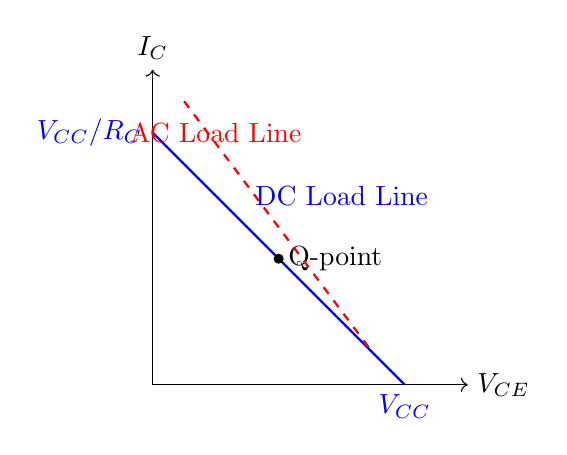
\begin{tikzpicture}[scale=0.8]
    \draw[->] (0,0) -- (5,0) node[right] {$V_{CE}$};
    \draw[->] (0,0) -- (0,5) node[above] {$I_C$};
    
    % DC Load Line
    \draw[thick, blue] (0,4) node[left] {$V_{CC}/R_C$} -- (4,0) node[below] {$V_{CC}$};
    \node[blue] at (3,3) {DC Load Line};

    % Q-point
    \filldraw (2,2) circle (2pt) node[right] {Q-point};
    
    % AC Load Line
    \draw[thick, red, dashed] (0.5, 4.5) -- (3.5, 0.5);
    \node[red] at (1, 4) {AC Load Line};
\end{tikzpicture}
\end{center}

\begin{itemize}
    \item \textbf{DC Load Line}: Shows all possible operating points under DC conditions.
    \begin{itemize}
        \item Equation: $I_C = (V_{CC} - V_{CE})/R_C$
        \item Endpoints: $(0, V_{CC}/R_C)$ and $(V_{CC}, 0)$
    \end{itemize}
    \item \textbf{AC Load Line}: Shows operating points during AC signal handling.
    \begin{itemize}
        \item Steeper Slope: Due to AC resistance being less than DC resistance.
        \item Centered at Q-point: The operating point established by biasing.
    \end{itemize}
\end{itemize}

\mnemonicbox{DC Draws Completely, AC Alters Course}
\end{solutionbox}

\questionmarks{2}{b}{4}
\textbf{Briefly explain bandwidth and gain-bandwidth product of an amplifier.}

\begin{solutionbox}
\textbf{Bandwidth and Gain-Bandwidth Product:}
Key specifications for amplifier frequency performance.

\begin{center}
\begin{tikzpicture}
    \node [gtu block, minimum width=3cm] (sys) {Amplifier\\Gain $\times$ Bandwidth};
    \draw [gtu arrow] (sys.west) ++(-1,0) -- (sys.west) node[midway, above] {Input};
    \draw [gtu arrow] (sys.east) -- ++(1,0) node[midway, above] {Output};
\end{tikzpicture}
\end{center}

\begin{center}
\captionof{table}{Frequency Parameters}
\begin{tabular}{|l|l|}
\hline
\textbf{Parameter} & \textbf{Description} \\ \hline
Bandwidth & Frequency range where gain drops by less than 3dB \\ \hline
Lower Cutoff ($f_1$) & Frequency where gain drops by 3dB at low end \\ \hline
Upper Cutoff ($f_2$) & Frequency where gain drops by 3dB at high end \\ \hline
Gain-Bandwidth Product & Product of gain and bandwidth, remains constant \\ \hline
\end{tabular}
\end{center}

\begin{itemize}
    \item \textbf{Bandwidth Formula}: $BW = f_2 - f_1$
    \item \textbf{Gain-Bandwidth}: Remains constant when gain changes ($A_v \times BW = C$).
    \item \textbf{Trade-off}: Higher gain means lower bandwidth.
\end{itemize}

\mnemonicbox{Better Bandwidth Gets Perfect Transmission}
\end{solutionbox}

\questionmarks{2}{c}{7}
\textbf{Explain frequency response of two stage RC coupled amplifier.}

\begin{solutionbox}
\textbf{Frequency Response of Two-Stage RC Coupled Amplifier:}

\begin{center}
\begin{tikzpicture}[node distance=3cm, auto]
    \node [gtu block] (S1) {Stage 1};
    \node [gtu block, right of=S1] (S2) {Stage 2};
    \node [left of=S1, node distance=2cm] (In) {Input};
    \node [right of=S2, node distance=2cm] (Out) {Output};

    \draw [gtu arrow] (In) -- (S1);
    \draw [gtu arrow] (S1) -- node[above] {RC Coupling} (S2);
    \draw [gtu arrow] (S2) -- (Out);
\end{tikzpicture}
\end{center}

\begin{center}
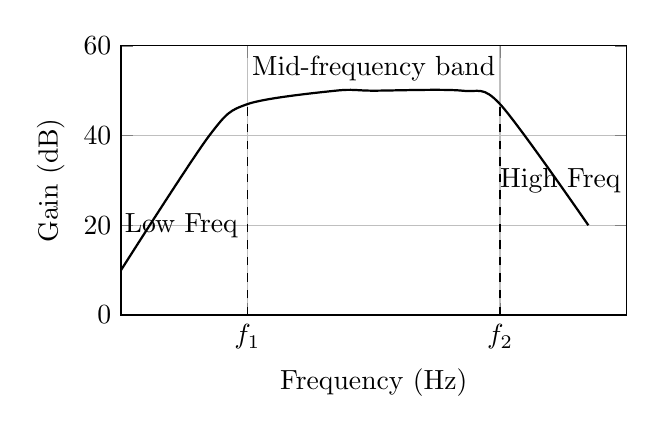
\begin{tikzpicture}
    \begin{semilogxaxis}[
        width=8cm, height=5cm,
        xlabel={Frequency (Hz)},
        ylabel={Gain (dB)},
        xmin=10, xmax=100000,
        ymin=0, ymax=60,
        xtick={100, 10000},
        xticklabels={$f_1$, $f_2$},
        grid=major
    ]
    \addplot[thick, smooth] coordinates {
        (10, 10) (50, 40) (100, 47) (500, 50) (1000, 50) (5000, 50) (10000, 47) (50000, 20)
    };
    \node at (axis cs: 1000, 55) {Mid-frequency band};
    \node at (axis cs: 30, 20) {Low Freq};
    \node at (axis cs: 30000, 30) {High Freq};
    \draw [dashed] (axis cs: 100, 0) -- (axis cs: 100, 47);
    \draw [dashed] (axis cs: 10000, 0) -- (axis cs: 10000, 47);
    \end{semilogxaxis}
\end{tikzpicture}
\end{center}

\begin{itemize}
    \item \textbf{Low Frequency Response}: Limited by coupling capacitors ($C_C$, $C_E$). Gain drops.
        \begin{itemize} \item Roll-off Rate: -20 dB/decade per stage. \end{itemize}
    \item \textbf{Mid Frequency Response}: Capacitors act as short circuits (coupling) or open (transistor internal). Gain is maximum and flat.
        \begin{itemize} \item Total Gain: Product of individual stage gains ($A_{total} = A_1 \times A_2$). \end{itemize}
    \item \textbf{High Frequency Response}: Limited by transistor inter-electrode capacitances. Gain drops.
\end{itemize}

\mnemonicbox{Low Couples Weakly, High Capacitance Blocks}
\end{solutionbox}

\questionmarks{2}{a}{3}
\textbf{Explain fixed bias circuit for transistor biasing.}

\begin{solutionbox}
\textbf{Fixed Bias Circuit:}
Fixed bias uses a single resistor connected to the base.

\begin{center}
\begin{circuitikz}[scale=0.9, transform shape]
    \draw (0,0) node[npn] (Q) {};
    \draw (Q.E) node[ground]{};
    \draw (Q.C) to[R, l=$R_C$] (0,2) -- (0,2.5) node[vcc]{$V_{CC}$};
    \draw (Q.B) to[short] (-1.5,0) to[R, l=$R_B$] (-1.5,2) -- (0,2);
    \draw (Q.B) to[short, -o] (-2,0) node[left] {$V_{in}$};
    \draw (Q.C) to[short, -o] (1,1) node[right] {$V_{out}$};
\end{circuitikz}
\end{center}

\begin{itemize}
    \item \textbf{Analysis}:
    \begin{itemize}
        \item Base Current: $I_B = (V_{CC} - V_{BE}) / R_B$
        \item Collector Current: $I_C = \beta \times I_B$
    \end{itemize}
    \item \textbf{Drawbacks}: Poor stability. $I_C$ varies directly with $\beta$ and temperature.
\end{itemize}

\mnemonicbox{Fix Bias, Face Burden (of instability)}
\end{solutionbox}

\questionmarks{2}{b}{4}
\textbf{Explain frequency response of single stage amplifier.}

\begin{solutionbox}
\textbf{Frequency Response of Single Stage Amplifier:}

\begin{center}
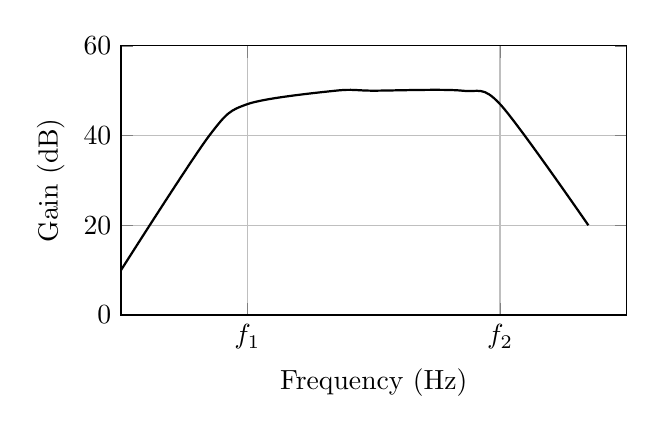
\begin{tikzpicture}
    \begin{semilogxaxis}[
        width=8cm, height=5cm,
        xlabel={Frequency (Hz)},
        ylabel={Gain (dB)},
        xmin=10, xmax=100000,
        ymin=0, ymax=60,
        xtick={100, 10000},
        xticklabels={$f_1$, $f_2$},
        grid=major
    ]
    \addplot[thick, smooth] coordinates {
        (10, 10) (50, 40) (100, 47) (500, 50) (1000, 50) (5000, 50) (10000, 47) (50000, 20)
    };
    \end{semilogxaxis}
\end{tikzpicture}
\end{center}

\begin{center}
\captionof{table}{Regions}
\begin{tabular}{|l|l|}
\hline
\textbf{Region} & \textbf{Characteristics} \\ \hline
Low Frequency & Gain drops due to coupling/bypass capacitors ($X_C$ is high) \\ \hline
Mid Frequency & Maximum and constant gain ($X_C \approx 0$ for ext caps, $\infty$ for int) \\ \hline
High Frequency & Gain decreases due to internal transistor capacitances \\ \hline
\end{tabular}
\end{center}

\begin{itemize}
    \item \textbf{Cutoff Frequencies}: Points where gain drops by 3dB from max.
    \item \textbf{Bandwidth}: $BW = f_2 - f_1$.
\end{itemize}

\mnemonicbox{Low Middle High - Capacitors Matter Here}
\end{solutionbox}

\questionmarks{2}{c}{7}
\textbf{Compare transformer coupled amplifier and RC coupled amplifier}

\begin{solutionbox}
\begin{center}
\captionof{table}{Comparison}
\begin{tabular}{|l|p{4cm}|p{4cm}|}
\hline
\textbf{Parameter} & \textbf{RC Coupled} & \textbf{Transformer Coupled} \\ \hline
Coupling Element & Resistor and Capacitor & Transformer \\ \hline
Frequency Response & Wide bandwidth & Limited bandwidth, poor low/high freq \\ \hline
Efficiency & Low (20-25\%) & Higher (50-60\%) \\ \hline
Size \& Weight & Small, lightweight & Bulky, heavy \\ \hline
Cost & Inexpensive & Expensive \\ \hline
Impedance Matching & Poor & Excellent \\ \hline
Application & Voltage amplification & Power amplification \\ \hline
\end{tabular}
\end{center}

\begin{center}
\begin{tikzpicture}[node distance=4cm, auto]
    \node [gtu block] (RC) {RC Coupled\\(R + C)};
    \node [gtu block, right of=RC] (Tx) {Transformer Coupled\\(Transformer)};
    \node [below of=RC, node distance=1.5cm] {Voltage Amp};
    \node [below of=Tx, node distance=1.5cm] {Power Amp};
\end{tikzpicture}
\end{center}

\mnemonicbox{RC Takes Breadth, Transformer Takes Power}
\end{solutionbox}

\questionmarks{3}{a}{3}
\textbf{Explain in brief Direct coupled amplifier.}

\begin{solutionbox}
\textbf{Direct Coupled Amplifier:}
Connects stages without coupling capacitors/transformers.

\begin{center}
\begin{tikzpicture}[node distance=3cm, auto]
    \node [gtu block] (S1) {Stage 1};
    \node [gtu block, right of=S1] (S2) {Stage 2};
    \node [left of=S1, node distance=2cm] (In) {Input};
    \node [right of=S2, node distance=2cm] (Out) {Output};

    \draw [gtu arrow] (In) -- (S1);
    \draw [gtu arrow] (S1) -- node[above] {Direct Wire} (S2);
    \draw [gtu arrow] (S2) -- (Out);
\end{tikzpicture}
\end{center}

\begin{itemize}
    \item \textbf{DC Signal Handling}: Can amplify very low frequencies (down to 0 Hz / DC).
    \item \textbf{No Coupling Elements}: Simple and cheap.
    \item \textbf{Drawbacks}: Thermal drift (shift in Q-point with temp) is passed to next stage.
\end{itemize}

\mnemonicbox{Directly Connected, Down to Complete zero frequency}
\end{solutionbox}

\questionmarks{3}{b}{4}
\textbf{Explain effects of emitter bypass capacitor and coupling capacitor on frequency response of an amplifier.}

\begin{solutionbox}
\textbf{Effects of Capacitors:}

\begin{center}
\captionof{table}{Capacitor Effects}
\begin{tabular}{|l|l|p{5cm}|}
\hline
\textbf{Component} & \textbf{Function} & \textbf{Effect on Response} \\ \hline
Emitter Bypass Cap ($C_E$) & Bypasses $R_E$ for AC & Increases gain at mid/high frequencies (prevents negative feedback). If removed, gain drops. \\ \hline
Coupling Cap ($C_C$) & Blocks DC, passes AC & Determines lower cutoff frequency. If too small, low freq gain drops. \\ \hline
\end{tabular}
\end{center}

\begin{center}
\begin{tikzpicture}[node distance=2.5cm, auto]
    \node [gtu block, align=center] (A) {Without Caps};
    \node [gtu block, right of=A, align=center] (B) {With Coupling\\Only};
    \node [gtu block, right of=B, align=center] (C) {With Coupling\\+ Bypass};
    \node [gtu block, right of=C, align=center] (D) {Ideal Response};

    \path [gtu arrow] (A) -- node[above, scale=0.7] {Low Gain} (B);
    \path [gtu arrow] (B) -- node[above, scale=0.7] {Med Gain} (C);
    \path [gtu arrow] (C) -- node[above, scale=0.7] {High Gain} (D);
\end{tikzpicture}
\end{center}

\mnemonicbox{Coupling Controls Lows, Bypass Boosts All}
\end{solutionbox}

\questionmarks{3}{c}{7}
\textbf{Draw Transistor Two Port Network and describe h-parameters for it. Write down advantages of hybrid parameters.}

\begin{solutionbox}
\textbf{Two-Port Network Model:}

\begin{center}
\begin{circuitikz}[scale=1]
    \draw (0,0) rectangle (4,2.5);
    \node at (2,1.25) {\large Two-Port Network};
    
    % Port 1
    \draw (-1.5, 2) to[short, i=$i_1$] (0, 2);
    \draw (-1.5, 0.5) to[short, o-] (0, 0.5);
    \draw (-1.5, 2) to[open, v=$v_1$] (-1.5, 0.5);
    
    % Port 2
    \draw (5.5, 2) to[short, i_=$i_2$] (4, 2);
    \draw (5.5, 0.5) to[short, o-] (4, 0.5);
    \draw (5.5, 2) to[open, v^=$v_2$] (5.5, 0.5);
\end{circuitikz}
\end{center}

\textbf{H-Parameters (Hybrid Parameters):}
\begin{enumerate}
    \item \textbf{$h_{11}$ ($h_i$)}: Input Impedance (Output Shorted) - $\frac{v_1}{i_1} |_{v_2=0}$
    \item \textbf{$h_{12}$ ($h_r$)}: Reverse Voltage Ratio (Input Open) - $\frac{v_1}{v_2} |_{i_1=0}$
    \item \textbf{$h_{21}$ ($h_f$)}: Forward Current Gain (Output Shorted) - $\frac{i_2}{i_1} |_{v_2=0}$
    \item \textbf{$h_{22}$ ($h_o$)}: Output Admittance (Input Open) - $\frac{i_2}{v_2} |_{i_1=0}$
\end{enumerate}

\textbf{Advantages:}
\begin{itemize}
    \item Easiliy Measured: $h_i, h_f$ at short circuit, $h_r, h_o$ at open circuit.
    \item Accurate Model: Good for small-signal analysis.
    \item Dimensions: Mixed (Ohm, Unitless, Mho).
\end{itemize}

\mnemonicbox{IRFO: Input, Reverse, Forward, Output}
\end{solutionbox}

\questionmarks{3}{a}{3}
\textbf{Draw frequency response ... and indicate ...}

\begin{solutionbox}
\textbf{Frequency Response Indicators:}

\begin{center}
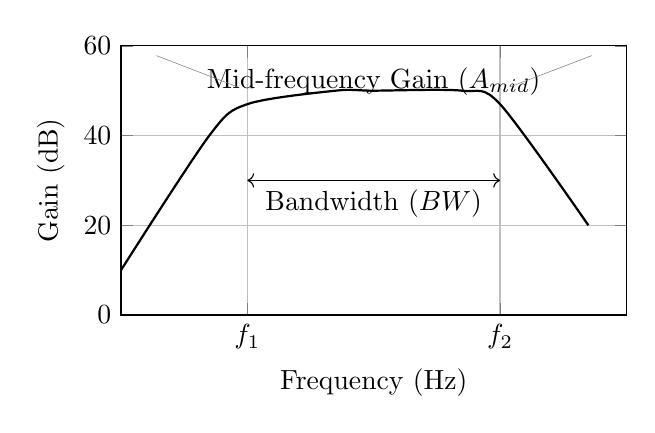
\begin{tikzpicture}
    \begin{semilogxaxis}[
        width=8cm, height=5cm,
        xlabel={Frequency (Hz)},
        ylabel={Gain (dB)},
        xmin=10, xmax=100000,
        ymin=0, ymax=60,
        xtick={100, 10000},
        xticklabels={$f_1$, $f_2$},
        grid=major
    ]
    \addplot[thick, smooth] coordinates {
        (10, 10) (50, 40) (100, 47) (500, 50) (1000, 50) (5000, 50) (10000, 47) (50000, 20)
    };
    
    % Annotations
    \draw[<->] (axis cs: 100, 30) -- (axis cs: 10000, 30) node[midway, below] {Bandwidth ($BW$)};
    \node at (axis cs: 1000, 52) {Mid-frequency Gain ($A_{mid}$)};
    \node at (axis cs: 100, 50) [pin=135:Lower Cutoff ($f_1$)] {};
    \node at (axis cs: 10000, 50) [pin=45:Upper Cutoff ($f_2$)] {};
    
    \end{semilogxaxis}
\end{tikzpicture}
\end{center}

\mnemonicbox{Lower Bandwidth Upper Makes Amplifier Response}
\end{solutionbox}

\questionmarks{3}{b}{4}
\textbf{Describe the transistor used as a tuned amplifier.}

\begin{solutionbox}
\textbf{Tuned Amplifier:}
Uses LC resonant circuits to selectively amplify specific frequencies (e.g., radio receivers).

\begin{center}
\begin{tikzpicture}[node distance=3cm, auto]
    \node [gtu block] (Amp) {Transistor Amp};
    \node [gtu block, right of=Amp] (LC) {LC Tank Circuit};
    \node [left of=Amp, node distance=2.5cm] (In) {Input};
    \node [right of=LC, node distance=2.5cm] (Out) {Output};

    \draw [gtu arrow] (In) -- (Amp);
    \draw [gtu arrow] (Amp) -- (LC);
    \draw [gtu arrow] (LC) -- (Out);
\end{tikzpicture}
\end{center}

\begin{itemize}
    \item \textbf{Resonance ($f_r$)}: $f_r = \frac{1}{2\pi\sqrt{LC}}$
    \item \textbf{Quality Factor (Q)}: Determines selectivity (Narrow BW = High Q).
    \item \textbf{Application}: Communication systems (Radio/TV).
\end{itemize}

\mnemonicbox{Tuning LC Selects Signals Precisely}
\end{solutionbox}

\questionmarks{3}{c}{7}
\textbf{Importance of h parameters ... Draw h-parameters circuit for CE amplifier.}

\begin{solutionbox}
\textbf{Importance:} Standardized, accurate, easily measured parameters for transistor analysis.

\textbf{CE Amplifier h-parameter Model:}

\begin{center}
\begin{circuitikz}[scale=1]
    \draw (0,0) to[short, o-] (1,0) to[R, l=$h_{ie}$] (3,0) to[cV, l=$h_{re}V_{ce}$] (3,-2) to[short, -o] (0,-2);
    \draw (0,0) node[left]{$B$};
    \draw (0,-2) node[left]{$E$};
    
    \draw (5,0) to[cI, l=$h_{fe}I_b$, invert] (5,-2);
    \draw (7,0) to[R, l=$\frac{1}{h_{oe}}$] (7,-2); 
    \draw (5,0) to[short, -o] (8,0) node[right]{$C$};
    \draw (5,-2) to[short, -o] (8,-2) node[right]{$E$};
    
    \draw (3,0) -- (8,0);
    \draw (3,-2) -- (8,-2);
\end{circuitikz}
\end{center}

\mnemonicbox{Input Resistance, Feedback Ratio, Forward Gain, Output Conductance}
\end{solutionbox}

\questionmarks{4}{a}{3}
\textbf{Describe the diode clipper circuit with necessary diagram.}

\begin{solutionbox}
\textbf{Diode Clipper:}
Limits/clips input signal above or below a reference level.

\begin{center}
\begin{circuitikz}
    \draw (0,0) to[sinusoidal voltage source, l=$V_{in}$] (0,2) to[R, l=$R$] (2,2) -- (4,2) to[short, -o] (5,2) node[right]{$V_{out}$};
    \draw (3,2) to[D*, l=$D$] (3,0);
    \draw (0,0) -- (5,0);
    \draw (3,0) -- (3,-0.5) node[ground]{};
\end{circuitikz}
\end{center}
\textit{(Diagram: Positive Clipper - clips positive half cycle)}

\mnemonicbox{Clip Portions Passing Preset Points}
\end{solutionbox}

\questionmarks{4}{b}{4}
\textbf{Explain Short note on LDR.}

\begin{solutionbox}
\textbf{LDR (Light Dependent Resistor):}
Resistance decreases as light intensity increases.

\begin{center}
\begin{tikzpicture}[node distance=2cm, auto]
    \node [gtu block] (LDR) {LDR};
    \node [left of=LDR, node distance=2cm] (Light) {Light $\uparrow$};
    \node [right of=LDR, node distance=3cm] (Res) {Resistance $\downarrow$};

    \draw [gtu arrow] (Light) -- (LDR);
    \draw [gtu arrow] (LDR) -- (Res);
\end{tikzpicture}
\end{center}

\begin{itemize}
    \item \textbf{Material}: Cadmium Sulfide (CdS).
    \item \textbf{Function}: Dark = High Resistance (M$\Omega$), Bright = Low Resistance (k$\Omega$).
    \item \textbf{Use}: Street lights, camera meters.
\end{itemize}

\mnemonicbox{Light Decreases Resistance}
\end{solutionbox}

\questionmarks{4}{c}{7}
\textbf{Explain Darlington pair and its applications.}

\begin{solutionbox}
\textbf{Darlington Pair:}
Two transistors connected in cascade (Super-Beta arrangement) for very high high current gain.

\begin{center}
\begin{circuitikz}
    \draw (0,0) node[npn] (Q1) {Q1};
    \draw (2,0) node[npn] (Q2) {Q2};
    \draw (Q1.C) -- (Q2.C) -- ++(0,1) node[vcc]{$C (Common)$};
    \draw (Q1.E) -- (Q2.B);
    \draw (Q1.B) -- ++(-0.5,0) node[left]{$B (Input)$};
    \draw (Q2.E) -- ++(0,-0.5) node[below]{$E (Output)$};
\end{circuitikz}
\end{center}

\textbf{Characteristics:}
\begin{itemize}
    \item \textbf{High Current Gain}: $\beta \approx \beta_1 \times \beta_2$.
    \item \textbf{High Input Impedance}: Good for buffering.
\end{itemize}

\textbf{Applications}: Power amplifiers, Relay drivers, Touch switches.

\mnemonicbox{Double Transistors Amplify Really Greatly}
\end{solutionbox}

\questionmarks{4}{a}{3}
\textbf{Describe the diode clamper circuit with necessary diagram.}

\begin{solutionbox}
\textbf{Diode Clamper:}
Shifts the DC level of a signal (adds DC offset) without changing its shape.

\begin{center}
\begin{circuitikz}
    \draw (0,0) to[sinusoidal voltage source] (0,2) to[C, l=$C$] (2,2) -- (4,2) to[short, -o] (5,2) node[right]{$V_{out}$};
    \draw (3,2) to[D*, l=$D$] (3,0);
    \draw (4,2) to[R, l=$R_L$] (4,0);
    \draw (0,0) -- (5,0);
\end{circuitikz}
\end{center}

\textit{Capacitor charges and acts as a battery, shifting the signal.}

\mnemonicbox{Clamps Peaks Down Consistently}
\end{solutionbox}

\questionmarks{4}{b}{4}
\textbf{Explain the working and applications of OLED.}

\begin{solutionbox}
\textbf{OLED (Organic LED):}
Display technology using organic films that emit light when current flows.

\begin{center}
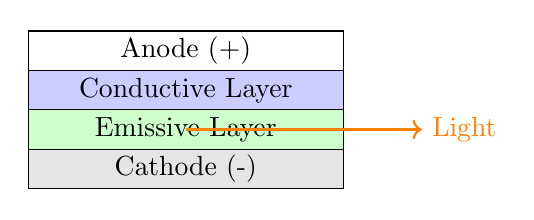
\begin{tikzpicture}
    % Stacked layers
    \draw[fill=gray!20] (0,0) rectangle (4,0.5) node[midway]{Cathode (-)};
    \draw[fill=green!20] (0,0.5) rectangle (4,1.0) node[midway]{Emissive Layer};
    \draw[fill=blue!20] (0,1.0) rectangle (4,1.5) node[midway]{Conductive Layer};
    \draw[fill=white] (0,1.5) rectangle (4,2.0) node[midway]{Anode (+)};
    \draw[->, thick, orange] (2, 0.75) -- (5, 0.75) node[right]{Light};
\end{tikzpicture}
\end{center}

\begin{itemize}
    \item \textbf{Structure}: Anode, Conductive, Emissive (Organic), Cathode.
    \item \textbf{Pros}: Self-emissive (no backlight), deeper blacks, flexible.
    \item \textbf{Uses}: Phones, TVs, Wearables.
\end{itemize}

\mnemonicbox{Organic Layers Emit Diode-light}
\end{solutionbox}

\questionmarks{4}{c}{7}
\textbf{Describe the transistor used as a relay driver.}

\begin{solutionbox}
\textbf{Relay Driver:}
Transistor acts as a switch to drive a high-current relay coil from a low-current logic signal.

\begin{center}
\begin{circuitikz}
    \draw (0,0) node[npn] (Q) {};
    \draw (Q.E) node[ground]{};
    \draw (Q.B) to[R, l=$R_B$] (-2,0) node[left]{Input Logic};
    
    % Relay Coil
    \draw (Q.C) -- (0,2) to[L, l=Relay Coil] (0,4) node[vcc]{$+V_{CC}$};
    
    % Flyback Diode
    \draw (1,2) to[D*, l=Flyback Diode] (1,4);
    \draw (0,2) -- (1,2);
    \draw (0,4) -- (1,4);
\end{circuitikz}
\end{center}

\begin{itemize}
    \item \textbf{Transistor}: Saturates (ON) to energize relay, Cutoff (OFF) to de-energize.
    \item \textbf{Flyback Diode}: Protects transistor from high voltage spike (Back EMF) when relay turns off.
\end{itemize}

\mnemonicbox{Tiny Regulates Driving Relays}
\end{solutionbox}

\questionmarks{5}{a}{3}
\textbf{Draw circuit diagram of a variable power supply using LM317 IC.}

\begin{solutionbox}
\textbf{LM317 Variable Supply:}

\begin{center}
\begin{circuitikz}
    \draw (0,0) node[draw, rectangle, minimum width=1.5cm, minimum height=1cm] (IC) {LM317};
    \node[left] at (IC.west) {IN};
    \node[right] at (IC.east) {OUT};
    \node[below] at (IC.south) {ADJ};
    
    \draw (IC.west) -- (-1,0) node[left]{$V_{in}$};
    \draw (IC.east) -- (2,0) node[right]{$V_{out}$};
    
    \draw (IC.east) to[short] (0.5,0) to[R, l=$R_1$] (0.5,-1.5) -- (IC.south);
    \draw (0.5,-1.5) to[vR, l=$R_2 (Pot)$] (0.5,-3) node[ground]{};
    
    \draw (IC.east) to[C, l=$C_2$] (2,0) -- (2,-3) node[ground]{};
\end{circuitikz}
\end{center}

Formula: $V_{out} = 1.25(1 + \frac{R_2}{R_1})$.

\mnemonicbox{LM317 Makes Voltage Adjustable}
\end{solutionbox}

\questionmarks{5}{b}{4}
\textbf{Explain working of UPS.}

\begin{solutionbox}
\textbf{UPS (Uninterruptible Power Supply):}
Provides backup power during mains failure.

\begin{center}
\begin{tikzpicture}[node distance=2.5cm, auto]
    \node [gtu block] (Rect) {Rectifier/\\Charger};
    \node [left of=Rect] (AC) {Mains AC};
    \node [gtu block, right of=Rect] (Bat) {Battery};
    \node [gtu block, right of=Bat] (Inv) {Inverter};
    \node [right of=Inv] (Load) {Load};

    \draw [gtu arrow] (AC) -- (Rect);
    \draw [gtu arrow] (Rect) -- (Bat);
    \draw [gtu arrow] (Bat) -- (Inv);
    \draw [gtu arrow] (Inv) -- (Load);
    
    % Bypass
    \draw [gtu arrow, dashed] (AC) to[out=90, in=90] node[midway, above]{Bypass Switch} (Load);
\end{tikzpicture}
\end{center}

\begin{itemize}
    \item \textbf{Normal}: Mains powers load + charges battery.
    \item \textbf{Backup}: Battery powers inverter -> load.
\end{itemize}

\mnemonicbox{Uninterrupted Power Supplied During Blackouts}
\end{solutionbox}

\questionmarks{5}{c}{7}
\textbf{Draw and explain SMPS block diagram.}

\begin{solutionbox}
\textbf{SMPS (Switch Mode Power Supply):}
Efficient power conversion using high-frequency switching.

\begin{center}
\begin{tikzpicture}[node distance=2cm, auto, scale=0.8, transform shape]
    \node [gtu block, align=center] (Filter1) {EMI\\Filter};
    \node [gtu block, right of=Filter1, node distance=2.5cm] (Rect1) {Rectifier\\\& Filter};
    \node [gtu block, right of=Rect1, node distance=2.5cm] (Switch) {HF\\Switch};
    \node [gtu block, right of=Switch, node distance=2.5cm] (Tx) {Transformer};
    \node [gtu block, right of=Tx, node distance=2.5cm] (Rect2) {Rectifier\\\& Filter};
    \node [below of=Switch] (PWM) {PWM Control};

    \draw [gtu arrow] (Filter1) -- (Rect1);
    \draw [gtu arrow] (Rect1) -- (Switch);
    \draw [gtu arrow] (Switch) -- (Tx);
    \draw [gtu arrow] (Tx) -- (Rect2);
    \draw [gtu arrow] (Rect2) -- ++(1.5,0) node[right]{DC Out};
    
    \draw [gtu arrow] (Rect2.south) |- (PWM.east);
    \draw [gtu arrow] (PWM) -- (Switch);
\end{tikzpicture}
\end{center}

\begin{itemize}
    \item \textbf{High Efficiency}: 70-90\% (transistor acts as switch, low power loss).
    \item \textbf{Compact}: High frequency allows smaller transformer.
\end{itemize}

\mnemonicbox{Switch Makes Power Stable}
\end{solutionbox}

\questionmarks{5}{a}{3}
\textbf{Draw circuit diagram for +15 v Power Supply using its IC and explain in brief}

\begin{solutionbox}
\textbf{+15V Supply (7815 IC):}

\begin{center}
\begin{circuitikz}
    \draw (0,0) node[draw, rectangle, minimum height=1cm] (IC) {7815};
    \node[left] at (IC.west) {IN};
    \node[right] at (IC.east) {OUT};
    \node[below] at (IC.south) {GND};
    
    \draw (IC.west) -- (-2,0) node[left]{Unregulated DC};
    \draw (IC.east) -- (2,0) node[right]{+15V Stable};
    \draw (IC.south) -- (0,-1) node[ground]{};
    
    \draw (-1.5,0) to[C, l=$C_1$] (-1.5,-1) node[ground]{};
    \draw (1.5,0) to[C, l=$C_2$] (1.5,-1) node[ground]{};
\end{circuitikz}
\end{center}

Uses 7815 linear regulator to output fixed +15V. $C_1, C_2$ filter noise.

\mnemonicbox{7815 Fixes Voltage To Fifteen}
\end{solutionbox}

\questionmarks{5}{b}{4}
\textbf{Explain working of solar battery charger circuits.}

\begin{solutionbox}
\textbf{Solar Charger:}

\begin{center}
\begin{tikzpicture}[node distance=3cm, auto]
    \node [gtu block] (Solar) {Solar Panel};
    \node [gtu block, right of=Solar] (Ctrl) {Charge\\Controller};
    \node [gtu block, right of=Ctrl] (Bat) {Battery};
    
    \draw [gtu arrow] (Solar) -- node[above]{DC} (Ctrl);
    \draw [gtu arrow] (Ctrl) -- (Bat);
    
    % Blocking Diode annotation
    \node[above of=Ctrl, node distance=1.5cm] (Label) {Blocking Diode prevents reverse flow};
    \draw[->, dotted] (Label) -- (Ctrl);
\end{tikzpicture}
\end{center}

Regulates solar voltage to safely charge battery. Prevents overcharge.

\mnemonicbox{Sun Charges Batteries Safely}
\end{solutionbox}

\questionmarks{5}{c}{7}
\textbf{Discuss comparison of linear regulated power supply with switch mode power supply.}

\begin{solutionbox}
\textbf{Comparison:}

\begin{center}
\captionof{table}{Linear vs SMPS}
\begin{tabular}{|l|l|l|}
\hline
\textbf{Parameter} & \textbf{Linear PS} & \textbf{SMPS} \\ \hline
Efficiency & Low (30-40\%) & High (70-90\%) \\ \hline
Size/Weight & Bulky/Heavy (50Hz Tx) & Compact/Light (HF Tx) \\ \hline
Noise & Low & High (Switching noise) \\ \hline
Complexity & Simple & Complex \\ \hline
App & Audio, Lab & PC, Adapters \\ \hline
\end{tabular}
\end{center}

\begin{center}
\begin{tikzpicture}[scale=0.8, transform shape]
    \node (L) at (0,0) [gtu block] {Linear: Drop Excess Voltage as Heat};
    \node (S) at (5,0) [gtu block] {SMPS: Chop Power Efficiently};
\end{tikzpicture}
\end{center}

\mnemonicbox{Linear Loves Low noise, Switching Saves Size}
\end{solutionbox}

\end{document}

